\documentclass[12pt]{article}

\usepackage[margin=0.8 in]{geometry}
\usepackage{amsmath}
\usepackage{amssymb}
\usepackage{macros}
\usepackage{mathtools}
\usepackage{enumerate}
\usepackage{verbatim}
\usepackage{amsthm}
\usepackage{hyperref}

\title{}
%\content{}



\let \proj \undefined
\renewcommand{\tr}{ \mathrm{tr}}
\DeclareMathOperator{\SU}{SU}
\DeclareMathOperator{\proj}{proj}
\newcommand{\sS}{\mathscr{S}}
\DeclareMathOperator{\comp}{comp}
\newcommand{\A}{\mathcal{A}}
\renewcommand{\D}{\mathcal{D}}
\renewcommand{\e}{\epsilon}
\newcommand{\et}{\tilde{\e}}
\newcommand{\vr}{\vec{r}}
\newcommand{\vF}{\vec{F}}
\newcommand{\triple}{\iiint_E f(x,y,z)dV}
\renewcommand{\lg}{\langle}
\newcommand{\rg}{\rangle}
\renewcommand{\i}{\vec{i}}
\renewcommand{\j}{\vec{j}}
\renewcommand{\k}{\vec{k}}
%\renewcommand{\k}{\vec{k}}

\newenvironment{solution}
  {\begin{proof}[Solution]}
  {\end{proof}
  
  }
\newtheorem{example}{Example}
\newtheorem{exercise}{Exercise}
\newtheorem{theorem}{Theorem}
\newtheorem{definition}{Definition}


\begin{document}
\subsection*{Vector fields}
What to know:
\begin{enumerate}
\item Be able to draw a few vectors of a vector field to understand what it looks like
\item Know the definition of conservative vector fields and potential functions
\end{enumerate}

Let's start with a real life example before getting technical: Think of a full bathtub once you remove the stopper: a vortex forms. If you throw little pieces of paper on the surface of the water near the hole, you'll see them move in a circular motion, and faster the closer they get to the hole. You can think of the pieces of paper as behaving similarly to the particles of the water, so we can observe that the particles have a velocity of different magnitudes and directions at different positions.

Another example: Think of this experiment you might have seen in elementary school: if you place iron fillings near a magnet, they align themselves according to the magnetic force exerted on them. The force becomes stronger near the poles, so they concentrate themselves more there. Again, we have a situation where the magnet exerts forces of different magnitude and direction at different points of the plane.

\begin{figure}[h]
\centering
\parbox{5cm}{
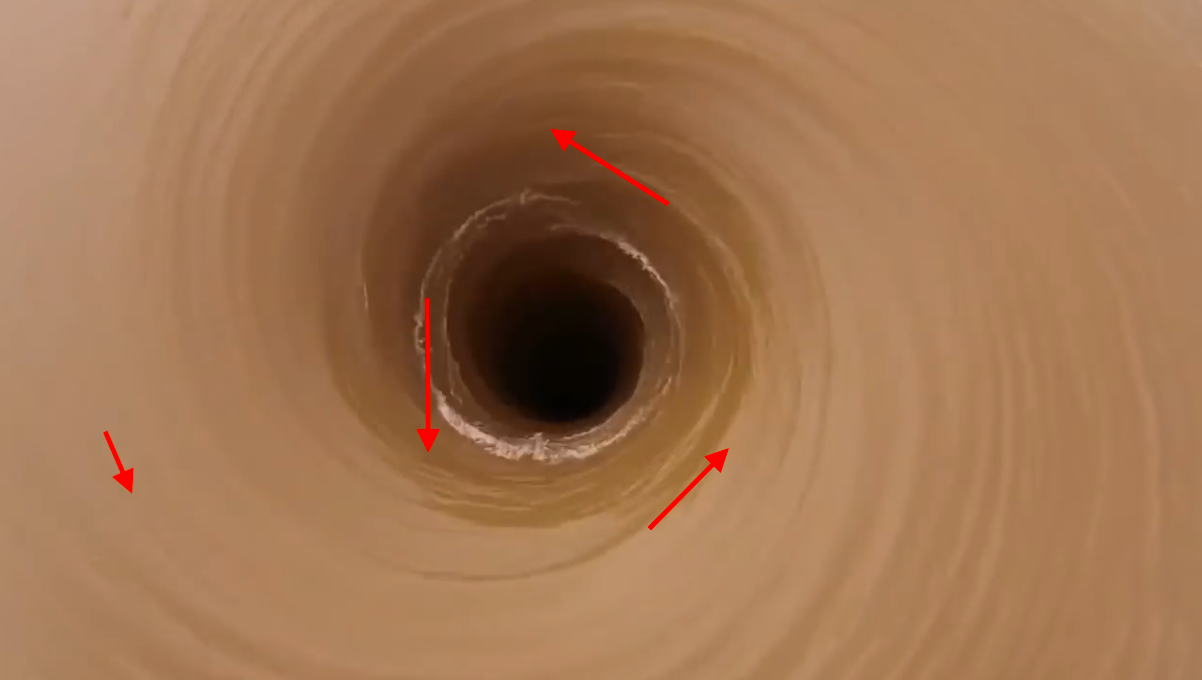
\includegraphics[width=5cm]{vortex.png}
\caption{A vortex}
\label{}}
\qquad
\begin{minipage}{5cm}
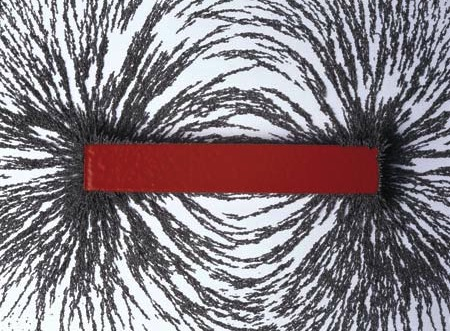
\includegraphics[width=5cm]{magnet.jpeg}
\caption{A magnet with iron fillings}
\label{fig:2figsB}
\end{minipage}
\end{figure}



Question: How can we describe such phenomena mathematically? Our goal is to assign to each point on the plane (or three dimensional space) an object that carries a magnitude and direction, and we've already seen such objects: vectors!

\begin{definition} If $D$ is a subset of $\R^2$, a\textbf{ vector field} on $D$ is a function that assigns to each point $(x,y)$ in $D$ a 2 dimensional vector $$\vF(x,y)=\langle P(x,y),Q(x,y)\rg=P(x,y)\i+Q(x,y)\j.$$
\end{definition}
Similarly, we have: 
\begin{definition} If $E$ is a subset of $\R^3$, a \textbf{vector field} on $E$ is a function that assigns to each point $(x,y,z)$ in $E$ a 3 dimensional vector $$\vF(x,y,z)=\langle P(x,y,z),Q(x,y,z),R(x,y,z)\rg=P(x,y,z)\i+Q(x,y,z)\j+R(x,y,z)\k.$$
\end{definition}

How we visualize vector fields: we draw arrows on the plane! In general, a computer is better than us at this, because it can draw much more vectors much more accurately, but we can usually get a feeling on what a vector field looks like by drawing vectors over 6-8 or so points. 

\begin{example}
Let $\vF(x,y)=\lg y,-x\rg$. We choose a few points and draw the corresponding vectors.
\begin{center}\begin{tabular}{|c|c|c|c|}
\hline 
Point & Vector & Point & Vector \\ 
\hline 
$(1,0)$ & $\lg 0, -1\rg$ & $(-1,0) $& $\lg 0,1\rg $\\	 
\hline 
$ (0,1)$& $\lg 1,0\rg $& $(0,-1)$ &  $\lg -1,0\rg $\\ 
\hline 
$(1,1)$& $\lg1,-1\rg$ & $(1,-1)$ & $\lg -1,-1\rg$ \\ 
\hline 
$(-1,1)$& $\lg 1,1\rg$ & $(-1,-1)$ & $\lg -1,1\rg$  \\ 
\hline 
\end{tabular} \end{center}


\begin{figure}[h]
\centering
\parbox{5cm}{
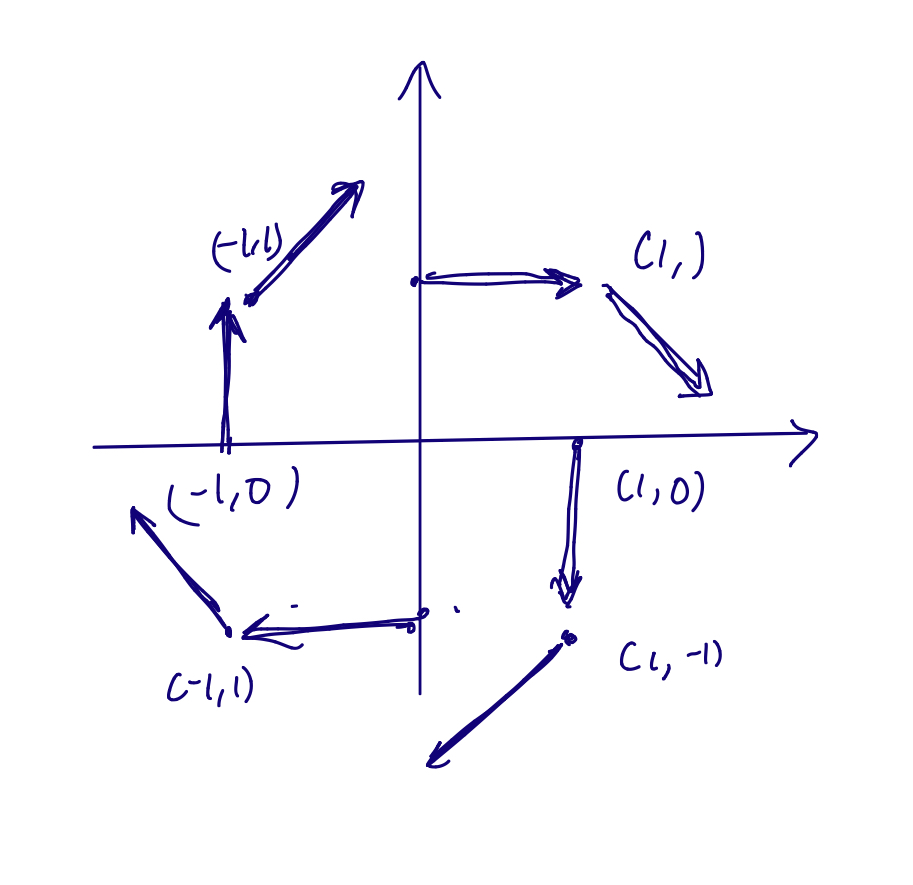
\includegraphics[width=5cm]{vf1.jpeg}
\caption{The vector field of the example}
\label{}}
\qquad
\begin{minipage}{5cm}
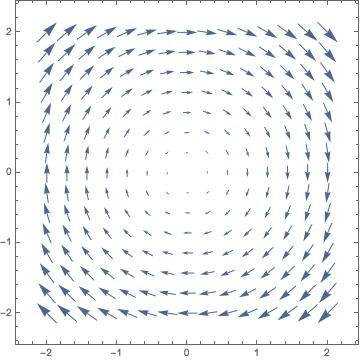
\includegraphics[width=5cm]{vf2.jpeg}
\caption{The same vector field plotted on Mathematica}
\label{fig:2figsB}
\end{minipage}
\end{figure}




\end{example}

\subsubsection*{Examples of vector fields}
\begin{enumerate}
\item We can use a vector field to describe the velocities of fluid particles (like in the bathtub case).
\item \textbf{Force fields}: in this case, each vector at each point corresponds to the force that is exerted to a test object, like in the case of the iron fillings in the example described above.
\item A special example of a force field is the \textbf{Gravitational vector field}. According to Newton's gravitational law, if an object with mass $M$ is located at the origin, then the gravitational force exerted on an object of mass $m$ located at $(x,y,z)$ is 
$$\vF(x,y,z)=-\frac{mMG}{(x^2+y^2+z^2)^{3/2}}\lg x,y,z\rg,$$ where $G=6.67\times 10^{-11}m^3kg^{-1}s^{-2}$ is the gravitational constant. Note that the Gravitational force \textbf{attracts} the objects closer to each other, which is reflected in the (-) sign.
\item Gradient fields: We've already seen that the gradient $\nabla f(x,y)$ of a differentiable function takes a point $(x,y)$ as input and gives a vector as output, so it can be understood as a vector field, called \textbf{gradient vector field} of $f$.
\end{enumerate}


\subsubsection*{Conservative vector fields}
We saw just before that from any differentiable function we can produce a vector field, the one given by its gradient. A natural question would be, are all vector fields the gradient vector field of a differentiable function? The answer is NO, but we have a name for those who are:
\begin{definition} A vector field $\vF$ on a set $D$ is called \textbf{conservative} if there exists a differentiable function $f(x,y)$ on $D$ so that $$\vF(x,y)=\nabla f(x,y).$$ In this case $f$ is called a \textbf{potential function } for $\vF$. 
\end{definition}
\begin{example} Find the gradient of $\dfrac{mMG}{(x^2+y^2+z^2)^{1/2}}$ and show that the gravitational vector field is conservative.
\end{example}
The importance of conservative vector fields will become more obvious in the next few weeks.



\subsubsection*{Integral curves of vector fields}
In the example of the bathtub, we have a vector field $\vF(x,y,z)$ that gives the velocity of each particle of the water. Knowing this vector field, can we predict the path a particle would follow knowing its initial position $(x_0,y_0,z_0)$?

If $\g(t)=(x(t),y(t),z(t))$ is this path, then the fact that $\vF$ is the velocity vector field for the particles of the fluid means exactly that 
$$\dot{\g}(t)=\vF(\g(t)),$$
or $$\lg\dot{x}(t),\dot{y}(t),\dot{z}(t)\rg=\vF(x(t),y(t),z(t)),$$
and under the initial condition $(x(0),y(0),z(0))=(x_0,y_0,z_0)$.
This is a first order Ordinary Differential Equation, and according to the Fundamental Theorem of ODE's, under some assumptions on $\vF$ it has a unique solution in an interval containing 0. However, practically finding this solution might be very difficult.

A curve satisfying this differential equation is called an \textbf{integral curve for $\vF$}.
\begin{example}
For the vector field $\vF(x,y,z)=\lg -y,x,z\rg$, the integral curve starting at (1,1,1) is given by $\g(t)=(x(t),y(t),z(t))$ 
\begin{align*}
x(t)&=\cos(t)-\sin(t)\\
y(t)&=\sin(t)+\cos(t)\\
z(t)&=e^t.
\end{align*} If you've taken Math 307 you can try to re-derive this, but you are not expected to be able to do this for this class! An animation of this example can be found here: \url{http://sites.math.washington.edu/~neptamin/324Au17/Mathematica/}
\end{example}
\end{document}



